\documentclass[12pt]{article}
\usepackage[left=1cm, right=1cm, top=2cm,bottom=1.5cm]{geometry} 

\usepackage[parfill]{parskip}
\usepackage[utf8]{inputenc}
\usepackage[T2A]{fontenc}
\usepackage[russian]{babel}
\usepackage{enumitem}
\usepackage[normalem]{ulem}
\usepackage{amsfonts, amsmath, amsthm, amssymb, mathtools}

\usepackage{tabularx}
\usepackage{hhline}

\usepackage{accents}
\usepackage{fancyhdr}
\pagestyle{fancy}
\renewcommand{\headrulewidth}{1.5pt}
\renewcommand{\footrulewidth}{1pt}

\usepackage{graphicx}
\usepackage[figurename=Рис.]{caption}
\usepackage{subcaption}
\usepackage{float}

%%Наименование папки откуда забирать изображения
\graphicspath{ {./images/} }

%%Изменение формата для ввода доказательства
\renewcommand{\proofname}{$\square$  \nopunct}
\renewcommand\qedsymbol{$\blacksquare$}

%%Изменение отступа на таблицах
\addto\captionsrussian{%
	\renewcommand{\proofname}{$\square$ \nopunct}%
}
%% Римские цифры
\newcommand{\RN}[1]{%
	\textup{\uppercase\expandafter{\romannumeral#1}}%
}

%% Для удобства записи
\newcommand{\MR}{\mathbb{R}}
\newcommand{\MC}{\mathbb{C}}
\newcommand{\MQ}{\mathbb{Q}}
\newcommand{\MN}{\mathbb{N}}
\newcommand{\MZ}{\mathbb{Z}}
\newcommand{\MTB}{\mathbb{T}}
\newcommand{\MTI}{\mathbb{I}}
\newcommand{\MI}{\mathrm{I}}
\newcommand{\MJ}{\mathrm{J}}
\newcommand{\MH}{\mathrm{H}}
\newcommand{\MT}{\mathrm{T}}
\newcommand{\MU}{\mathcal{U}}
\newcommand{\MV}{\mathcal{V}}
\newcommand{\MB}{\mathcal{B}}
\newcommand{\MF}{\mathcal{F}}
\newcommand{\MW}{\mathcal{W}}
\newcommand{\ML}{\mathcal{L}}
\newcommand{\MP}{\mathcal{P}}
\newcommand{\VN}{\varnothing}
\newcommand{\VE}{\varepsilon}

\theoremstyle{definition}
\newtheorem{defn}{Опр:}
\newtheorem{rem}{Rm:}
\newtheorem{prop}{Утв.}
\newtheorem{exrc}{Упр.}
\newtheorem{lemma}{Лемма}
\newtheorem{theorem}{Теорема}
\newtheorem{corollary}{Следствие}

\newenvironment{cusdefn}[1]
{\renewcommand\thedefn{#1}\defn}
{\enddefn}

\DeclareRobustCommand{\divby}{%
	\mathrel{\text{\vbox{\baselineskip.65ex\lineskiplimit0pt\hbox{.}\hbox{.}\hbox{.}}}}%
}
%Короткий минус
\DeclareMathSymbol{\SMN}{\mathbin}{AMSa}{"39}
%Длинная шапка
\newcommand{\overbar}[1]{\mkern 1.5mu\overline{\mkern-1.5mu#1\mkern-1.5mu}\mkern 1.5mu}
%Функция знака
\DeclareMathOperator{\sgn}{sgn}

%Функция ранга
\DeclareMathOperator{\rk}{\text{rk}}

%Обозначение константы
\DeclareMathOperator{\const}{\text{const}}

\DeclareMathOperator*{\dsum}{\displaystyle\sum}
\newcommand{\ddsum}[2]{\displaystyle\sum\limits_{#1}^{#2}}

%Интеграл в большом формате
\DeclareMathOperator{\dint}{\displaystyle\int}
\newcommand{\ddint}[2]{\displaystyle\int\limits_{#1}^{#2}}
\newcommand{\ssum}[1]{\displaystyle \sum\limits_{n=1}^{\infty}{#1}_n}

\newcommand{\smallerrel}[1]{\mathrel{\mathpalette\smallerrelaux{#1}}}
\newcommand{\smallerrelaux}[2]{\raisebox{.1ex}{\scalebox{.75}{$#1#2$}}}

\newcommand{\smallin}{\smallerrel{\in}}
\newcommand{\smallnotin}{\smallerrel{\notin}}

\newcommand*{\medcap}{\mathbin{\scalebox{1.25}{\ensuremath{\cap}}}}%
\newcommand*{\medcup}{\mathbin{\scalebox{1.25}{\ensuremath{\cup}}}}%

\makeatletter
\newcommand{\vast}{\bBigg@{3.5}}
\newcommand{\Vast}{\bBigg@{5}}
\makeatother

%Промежуточное значение для sup\inf, поскольку они имеют разную высоту
\newcommand{\newsup}{\mathop{\smash{\mathrm{sup}}}}
\newcommand{\newinf}{\mathop{\mathrm{inf}\vphantom{\mathrm{sup}}}}

%Скалярное произведение
\newcommand{\inner}[2]{\left\langle #1, #2 \right\rangle }
\newcommand{\linsp}[1]{\left\langle #1 \right\rangle }

%Подпись символов снизу
\newcommand{\ubar}[1]{\underaccent{\bar}{#1}}

%% Шапка для букв сверху
\newcommand{\wte}[1]{\widetilde{#1}}
\newcommand{\wht}[1]{\widehat{#1}}

%%Трансформация Фурье
\newcommand{\fourt}[1]{\mathcal{F}\left(#1\right)}
\newcommand{\ifourt}[1]{\mathcal{F}^{-1}\left(#1\right)}

%%Символ вектора
\newcommand{\vecm}[1]{\overrightarrow{#1\,}}

%%Пространстов матриц
\newcommand{\mat}[2]{Mat_{#1\times #2}}


%%Взятие в скобки, модули и норму
\newcommand{\parfit}[1]{\left( #1 \right)}
\newcommand{\modfit}[1]{\left| #1 \right|}
\newcommand{\sqparfit}[1]{\left\{ #1 \right\}}
\newcommand{\normfit}[1]{\left\| #1 \right\|}

%%Функция для обозначения равномерной сходимости по множеству
\newcommand{\uconv}[1]{\overset{#1}{\rightrightarrows}}
\newcommand{\uconvm}[2]{\overset{#1}{\underset{#2}{\rightrightarrows}}}


%%Функция для обозначения нижнего и верхнего интегралов
\def\upint{\mathchoice%
	{\mkern13mu\overline{\vphantom{\intop}\mkern7mu}\mkern-20mu}%
	{\mkern7mu\overline{\vphantom{\intop}\mkern7mu}\mkern-14mu}%
	{\mkern7mu\overline{\vphantom{\intop}\mkern7mu}\mkern-14mu}%
	{\mkern7mu\overline{\vphantom{\intop}\mkern7mu}\mkern-14mu}%
	\int}
\def\lowint{\mkern3mu\underline{\vphantom{\intop}\mkern7mu}\mkern-10mu\int}


\begin{document}
\lhead{Линейная алгебра и геометрия}
\chead{Тимашев Д.А.}
\rhead{Лекция - 2}
\section*{Замена координат в векторных пространствах}
\subsection*{Геометрический взгляд на векторные пространства}
На прошлой лекции мы доказали, что все конечномерные векторные пространства одной и той же размерности изморфны между собой. Казалось бы тогда достаточно взять какое-то одно пространство и всё про него понять. Однако такой подход не всегда удобен, поскольку в пространстве строк или столбцов в арифметическом пространстве есть некоторая выделенная система координат, стандартный базис, координатами в котором являются просто элементы столбца, которая не всегда удобна для решения задач. Поэтому правильнее смотреть на векторные пространства и объекты линейной алгебры, которые живут в этих пространствах геометрически, независимо от системы координат.

\subsection*{Матрицы перехода из одного базиса в другой}
Пусть $V$ - векторное пространство над полем $K$, $\dim{V} = n < \infty$, $e = (e_1, \dotsc, e_n)$ - базис $V$, одновременно возьмем в $V$ какой-то другой базис $e' = (e'_1, \dotsc, e'_n)$. 

Хотелось бы понять, как эти два базиса друг с другом связаны? Пусть мы будем называть $e$ - старым базисом, а $e'$ - новым базисом и попытаемся понять, что происходит при переходе от старого базиса к новому. Поскольку $e'_j \in V$, то он раскладывается по старому базису:
$$
	\forall j = 1, \dotsc, n, \, e'_j = c_{1j}e_1 + c_{2j}e_2 + \dotsc + c_{nj}e_n = \ddsum{i = 1}{n}c_{ij}e_i
$$
Из коэффициентов $\{c_{ij}\}$ можно составить квадратную матрицу размера $n \times n$:
$$
	C = 
	\begin{pmatrix}
		c_{11} & \dotsc & c_{1j} & \dotsc  & c_{1n} \\
		c_{21} & \dotsc & c_{2j} & \dotsc & c_{2n}\\
		\vdots & \ddots & \vdots & \ddots & \vdots\\
		c_{n1} & \dotsc & c_{nj} & \dotsc & c_{nn}
	\end{pmatrix}
$$
\begin{defn}
	Матрица $C$ называется \uwave{матрицей перехода} от базиса $e$ к базису $e'$. 
\end{defn}
В первом столбце матрицы $C$ записаны координаты вектора $e'_1$, во втором координаты $e'_2$ и так далее до вектора $e'_n$ в базисе $e$. Матрица перехода однозначно определяет новый базис $\Rightarrow$ чтобы задать новый базис, надо задать матрицу перехода к нему. Будем обозначать переход от $e$ к $e'$ так: 
$$
	e \xrightarrow[]{C}e'
$$

\textbf{\uline{Матричная запись}}: Если $e'_j = 
	\begin{pmatrix}
		e_1 & \dotsc & e_n
	\end{pmatrix}{\cdot}
	\begin{pmatrix}
		c_{1j}\\
		\vdots\\
		c_{nj}
	\end{pmatrix} $, то:
$$
	e' = 
	\begin{pmatrix}
		e'_1 & \dotsc & e'_n
	\end{pmatrix} = 
	\begin{pmatrix}
		e_1 & \dotsc & e_n
	\end{pmatrix}{\cdot}
	\begin{pmatrix}
		c_{11} & \dotsc & c_{1j} & \dotsc  & c_{1n} \\
		c_{21} & \dotsc & c_{2j} & \dotsc & c_{2n}\\
		\vdots & \ddots & \vdots & \ddots & \vdots\\
		c_{n1} & \dotsc & c_{nj} & \dotsc & c_{nn}
	\end{pmatrix} = e{\cdot}C \Rightarrow e' = e{\cdot}C
$$

\newpage
\subsection*{Свойства матрицы перехода}

\begin{enumerate}[label=\arabic*)]
	\item Матрица перехода невырождена и наоборот, любая невырожденная матрица $C \in \mat{n}{n}(K)$ размера $n \times n$ над полем $K$ является матрицей перехода от исходного базиса к некоторому новому;
	\begin{proof}\hfill\\
		$(\Rightarrow)$ Пусть $e \xrightarrow[]{C} e'$. Выбор базиса $e$ в пространстве $V$ задает изоморфизм: $V \simeq K^n$, при котором каждому вектору соответствует столбец координат этого вектора в базисе $e$. В частности:
		$$
			\forall j = \overline{1, n}, \, e'_j \longleftrightarrow 
			\begin{pmatrix}
				c_{1j}\\
				\vdots \\
				c_{nj}
			\end{pmatrix}
		$$
		Векторы $e'_1, \dotsc e'_n$ - линейно независимы, поскольку образуют базис $\Rightarrow$ столбцы матрицы перехода $C$ тоже будут линейно независимы $\Rightarrow$ матрица будет невырождена по определению.
		
		$(\Leftarrow)$ Пусть $C$ - невырожденная матрица $n \times n \Rightarrow$ её столбцы линейно независимы $\Rightarrow$ образуют базис пространства столбцов $K^n$, иначе это была бы не максимальная система линейно независимых столбцов $\Rightarrow$ в $n$-мерном пространстве столбцов нашлась бы линейно независимая система столбцов из $(n+1)$ столбца $\Rightarrow$ противоречие с основной леммой о линейной зависимости. Следовательно, при изоморфизме $K^n \simeq V$, векторы $e'_j$, соответствующие столбцам матрицы $C$:
		$$
			\forall j = \overline{1, n}, \, e'_j = \ddsum{i = 1}{n}c_{ij}e_i = 
			\begin{pmatrix}
				e_1 & \dotsc & e_n
			\end{pmatrix}{\cdot}
			\begin{pmatrix}
				c_{1j}\\
				\vdots\\
				c_{nj}
			\end{pmatrix}
		$$
		образуют базис пространства $V$, поскольку их $n$ штук и они линейно независимы. И переход от старого базиса $e$ к новому базису $e'$ осуществляется с помощью матрицы $C$:
		$$
			 e \xrightarrow[]{C} e' = \begin{pmatrix}
				e'_1 & \dotsc & e'_n
			\end{pmatrix}
		$$
	\end{proof}
	\item Если верно $e \xrightarrow[]{C} e'$, то $e' \xrightarrow[]{C^{-1}}e$ (обратный переход);
	\begin{proof}
		Пусть будет верно:
		$$
			e \xrightarrow[]{C} e' \xrightarrow[]{C'} e
		$$
		Тогда по свойству $3)$ справедливо:
		$$
			e = e{\cdot}C{\cdot}C' \Rightarrow C{\cdot}C' = I
		$$
		Аналогично:
		$$
			e' \xrightarrow[]{C'} e \xrightarrow[]{C} e' \Rightarrow e' = e'{\cdot}C'{\cdot}C \Rightarrow C'{\cdot}C = I
		$$
		Таким образом, $C'{\cdot}C = C{\cdot}C' = I \Leftrightarrow C' = C^{-1}$ по определению.
	\end{proof}
	\item Если верно $e \xrightarrow[]{C} e', \, e' \xrightarrow[]{C'} e''$, то $e \xrightarrow[]{C{\cdot}C'} e''$ (транзитивность);
	\begin{proof}
		Если область, откуда берутся коэффициенты тех или иных матриц, имеет ассоциативное умножение, то и умножение матриц автоматически будет ассоциативно. Тогда:
		$$
			e' = e{\cdot}C, \, e'' = e'{\cdot}C' \Rightarrow e'' = e{\cdot}C{\cdot}C' 
		$$
	\end{proof}
\end{enumerate}

\subsection*{Преобразование координат}
Пусть $x \in V$, разложим по старому базису:
$$
	x = x_1 e_1 + \dotsc + x_n e_n  = e{\cdot}X = 
	\begin{pmatrix}
		e_1 & \dotsc & e_n	
	\end{pmatrix}{\cdot}
	\begin{pmatrix}
		x_1 \\
		\vdots\\
		x_n
	\end{pmatrix}
$$
Разложим $x$ по новому базису:
$$
	x = x'_1e'_1 + \dotsc + x'_n e'_n = e'{\cdot}X' =
	\begin{pmatrix}
		e'_1 & \dotsc & e'_n	
	\end{pmatrix}{\cdot}
	\begin{pmatrix}
		x'_1 \\
		\vdots\\
		x'_n
	\end{pmatrix} = e{\cdot}\underbrace{C{\cdot}X'}_{\in K^n}
$$
Поскольку разложение вектора $x$ через базис $e$ единственно, то мы получаем, что выражение старых координат через новые будет иметь следующий вид: 
$$
	X = C{\cdot}X'
$$
Аналогично для выражения новых координат через новые, достаточно домножить это равенство на обратную матрицу перехода слева:
$$
	X = C{\cdot}X' \Rightarrow C^{-1}{\cdot}X = C^{-1}{\cdot}C{\cdot}X' = I{\cdot}X' = X' 
$$
\begin{prop}
	Для любого $x \in V$ при замене базиса от $e$ к $e'$ с помощью матрицы перехода, преобразование координат будет иметь следующий вид:
	$$
		X = C{\cdot}X', \quad X' = C^{-1}{\cdot}X
	$$
\end{prop}

\section*{Подпространства}
Пусть $V$ - векторное пространство над полем $K$.
\begin{defn}
	\uwave{Подпространством} называется непустое подмножество $U \subseteq V, \, U \neq \VN$, для которого:
	\begin{enumerate}[label=\arabic*)]
		\item $\forall u,v \in U, \, u + v \in U$;
		\item $\forall u \in U, \, \forall \lambda \in K, \, \lambda{\cdot}u \in U$;
	\end{enumerate}
	то есть замкнутость, относительно тех операций, которые мы умеем делать над векторами.
\end{defn}
\begin{rem}
	Если $v_1, \dotsc, v_m \in U$, тогда их линейные комбинации также принадлежат подпространству $U$: 
	$$
		v_1, \dotsc, v_m \in U \Rightarrow \forall \lambda_1, \dotsc, \lambda_m \in K, \, v = \lambda_1 v_1 + \dotsc + \lambda_m v_m \in U
	$$
\end{rem}
\begin{prop}
	В любом подпространстве $U \subseteq V$ всегда есть конкретный вектор: $\vecm{0} \in U$.
\end{prop}
\begin{proof}
	$$
		U \neq \VN \Rightarrow u \in U \Rightarrow  0{\cdot}u = \vecm{0} \in U 
	$$
\end{proof}
\begin{rem}
	Подпространство $U$ само является векторным пространством, относительно операций на $V$, ограниченных на $U$.
\end{rem}

\subsection*{Примеры векторных подпространств}
\begin{enumerate}[label=(\arabic*)]
	\item $U = \{0\} \subseteq V$ - наименьшее подпространство в пространстве $V$;
	\item $U = V \subseteq V$ - наибольшее подпространство в пространстве $V$;
	\item $V = \{\text{геом. векторы в пространстве}\}$, $U = \{\text{геом. векторы, параллельные плоскости } P\} \subseteq V$;
	\begin{figure}[H]
		\centering
		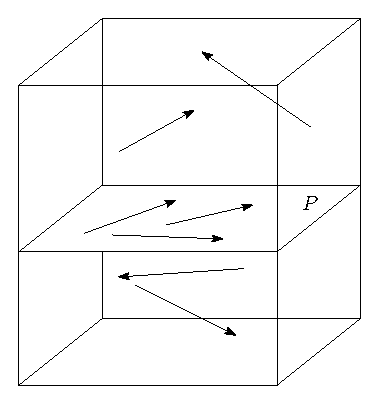
\includegraphics[width=0.25\textwidth]{LAL2_1.eps}
		\caption{Подпространство в геометрическом пространстве.}
		\label{2_1}
	\end{figure}
	Когда мы складываем векторы данной плоскости и умножаем их на вещественные числа мы снова получаем векторы этой плоскости $\Rightarrow$ это векторное подпространство;
	\item $V = \MF(\MR,\MR)$ - все функции на вещественной прямой с вещественными значениями, \\
	$U = C(\MR,\MR)$ - множество непрерывных функций на вещественной прямой с вещественными значениями. Сумма двух непрерывных функций - непрерывная функция, если домножить непрерывную функцию на число, то получим снова непрерывную функцию $\Rightarrow C(\MR,\MR)$ - подпространство;
\end{enumerate}

\subsection*{Конструкции подпространств}
$1)$ Пусть $S \subseteq V$ - система векторов.
\begin{defn}
	\uwave{Линейная оболочка} $\linsp{S}$ системы векторов $S \subseteq V$ это множество всевозможных линейных комбинаций векторов из системы $S$:
	$$
		U = \langle S \rangle = \left\{v = \lambda_1 v_1 + \dotsc+ \lambda_m v_m \mid i = \overline{1,m}, \, v_i \in S, \, \lambda_i \in K\right\}
	$$ 
\end{defn}
Легко понять, что $U = \linsp{S}$ это подпространство. Пусть $S = (v_1, \dotsc, v_m)$, тогда: 
\begin{enumerate}[label=\arabic*)]
	\item $\forall u,v \in \linsp{S}, \, u + w = \lambda_1 v_1 + \dotsc \lambda_m v_m + \mu_1 v_1 + \dotsc + \mu_m v_m = (\lambda_1 + \mu_1)v_1 + \dotsc + (\lambda_m + \mu_m)v_m \in \linsp{S}$;
	\item $\forall u \in \linsp{S}, \, \forall \lambda \in K, \, \lambda{\cdot}u = \lambda {\cdot}( \mu_1v_1 + \dotsc + \mu_m v_m) = (\lambda{\cdot}\mu_1)v_1 + \dotsc + (\lambda{\cdot}\mu_m)v_m \in \linsp{S}$;
\end{enumerate}

Общепринято считать, что при отсутствии слагаемых в сумме её значение равно $0$. В том числе допускается отсутствие слагаемых, то есть: $S = \VN \Rightarrow \linsp{S} = \{0\} \Rightarrow$ это гарантирует непустоту. Более того, линейная оболочка это подпространство - наименьшее, содержащее систему векторов $S$, поскольку если подпространство содержит систему векторов $S$, то оно должно содержать и все линейные комбинации векторов из системы $S$. Заметим, что система векторов $S$ \uline{порождает} свою линейную оболочку $\linsp{S}$ по определению с прошлой лекции.

\newpage
$2)$ $V = K^n$ - арифметическое пространство, пространство столбцов. Рассмотрим ОСЛУ (однородную систему линейных уравнений):
$$
	\left\{
	\begin{array}{ccccccc}
		a_{11}x_1 & + & \dotsc & + & a_{1n}x_n & = & 0 \\
		\vdots & \vdots & \ddots & \vdots & \vdots & \vdots & \vdots \\
		a_{m1}x_1 & + & \dotsc & + & a_{mn}x_n & = & 0 
	\end{array}
	\right.
$$
И рассмотрим множество решение ОСЛУ $= U$. Решением ОСЛУ называется набор (строка или столбец), состоящий из значений неизвестных, которые при подстановке вместо неизвестных дают верное равенство, то есть это некое подмножество в пространстве столбцов. 

В $1$-ом семестре доказывали, что множество решений ОСЛУ является подпространством в пространстве столбцов. Размерность этого пространства равна размерности всего пространства столбцов минус ранг матрицы коэффициентов.

\begin{rem}
	По изоморфности, задание подпространства с помощью ОСЛУ также работает в любых других конечномерных пространствах.
\end{rem}

$3)$ Пусть $U_1, \dotsc, U_m \subseteq V$ - набор подпространств $\Rightarrow U = U_1 \cap \dotsc \cap U_m$, будет ли пересечение подпространством? Очевидно, что $\vecm{0}\in U \Rightarrow$ пересечение не пусто. Замкнутость относительно операций также сохраняется: поскольку векторы лежат в каждом из $U_i$, то и результат операции будет лежать в каждом из $U_i \Rightarrow$ результат будет лежать в пересечении. 

\begin{rem}
	Заметим, что $U_1 \cup \dotsc \cup U_n$ вообще говоря, не будет подпространством.
\end{rem}

\textbf{\uline{Пример}}: Рассмотрим пространство $V$ геометрических векторов на плоскости. Для простоты будем откладывать векторы от какой-то начальной точки. Возьмем в этой плоскости две прямых $U_1$ и $U_2$, проходящих через начало координат, и рассмотрим векторы на этих прямых. 
\begin{figure}[H]
	\centering
	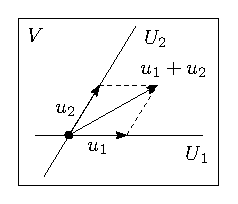
\includegraphics[width=0.2\textwidth]{LAL2_2.eps}
	\caption{Объединение подпространств не подпространство.}
	\label{2_2}
\end{figure}
Векторы на первой прямой и на второй прямой будут образовывать подпространства в $V$, а их объединение подпространством уже не будет: 
$$
	u_1 \in U_1, \, u_2 \in U_2, \, u_1,u_2 \neq \VN \Rightarrow u_1 + u_2 \not\in U_1 \cup U_2
$$
В результате, $U_1 \cup U_2$ - не подпространство $V$. Но с этим можно побороться.
\newpage
$4)$ Пусть $U_1,\dotsc, U_m \subseteq V$ - подпространства пространства $V$.
\begin{defn}
	\uwave{Суммой подпространств} называется линейная оболочка их объединения, то есть наименьшее подпространство, содержащее каждое из них:
	$$
		U_1 + \dotsc + U_m = \linsp{U_1 \cup \dotsc \cup U_m} = \left\{v = u_1 + \dotsc + u_m\mid \forall i = \overline{1,m}, \, u_i \in U_i\right\}
	$$
\end{defn}
Линейная оболочка любой системы векторов является подпространством, а сумма подпространств это линейная оболочка объединения подпространств $\Rightarrow$ также будет подпространством.
В предыдущем примере сумма: $U_1 + U_2 = V \Rightarrow$ очевидно является подпространством.

\begin{prop}
	Пусть $\dim{V} < \infty$, $U\subseteq V$ - подпространство. Тогда:
	\begin{enumerate}[label=\arabic*)]
		\item $\dim{U} \leq \dim{V}$;
		\item Любой базис $(e_1,\dotsc, e_m)$ подпространства $U$ можно дополнить до базиса $(e_1, \dotsc, e_m, e_{m+1}, e_n)$ пространства $V$;
		\item $\dim{U} = \dim{V}$ возможно только при $U = V$
	\end{enumerate}
\end{prop}
\begin{proof}
	Пусть $\dim{V} = n$.
	\begin{enumerate}[label=\arabic*)]
		\item По основной лемме о линейной зависимости, в пространстве $V$ не существует линейно независимых систем из больше чем $n$ векторов. Иначе, больше чем $n$ векторов выражается через $n$ векторов и большее число векторов - линейно независимы $\Rightarrow$ поскольку нельзя выбрать больше чем $n$ линейно независимых векторов в пространстве $U$, то $U$ также конечномерно и верно: $\dim{U} \leq \dim{V}$;
		\item Пусть $(e_1,\dotsc, e_m)$ - базис $U$, $m \leq n$. По определению базиса, эти векторы образуют максимальную линейно независимую систему в $U$, а во всём $V$ они образуют линейно независимую систему, но может быть не максимальную. Если система не максимальна, то можно дополнить $(e_1,\dotsc,e_m)$ до максимальной линейно независимой системы $(e_1,\dotsc,e_m,e_{m+1},\dotsc, e_n)$ векторов в $V$: 
		$$
			(e_1,\dotsc,e_m) \to (e_1,\dotsc,e_m,e_{m+1},\dotsc, e_n)
		$$
		Мы можем добавить лишь конечное число векторов, потому что линейно независимых систем из больше чем $n$ векторов в $V$ не существует $\Rightarrow$ это и есть искомый базис; 
		\item Если $\dim{U} = m = n = \dim{V} \Rightarrow (e_1, \dotsc, e_m)$ - это базис одновременно и для $U$, и для $V \Rightarrow U = V$;
	\end{enumerate}

\end{proof}
\begin{defn}
	Базис $(e_1, \dotsc, e_n)$ пространства $V$ \uwave{согласован} с подпространством $U$, если векторы $\left(e_{i_1}, \dotsc, e_{i_m}\right)$ это базис $U$ для некоторых $i_1, \dotsc, i_m \in \{1,\dotsc,n\}$. 
\end{defn}

\begin{corollary}
	В конечномерном векторном пространстве $V$ для любого подпространства $U$ существует согласованный с ним базис пространства $V$. 
\end{corollary}
\begin{proof}
	Этот базис построен в пункте $2)$ утверждения $3$.
\end{proof}
\begin{rem}
	Без ограничения общности, можно считать, что $(e_1,\dotsc, e_m)$ - базис $U$.
\end{rem}
В координатах в согласованном базисе: $U = \{x \in V \mid x_{m+1} = \dotsc = x_n = 0\}$, то есть задается ОСЛУ.
\newpage
\begin{theorem}
	Пусть $\dim{V} < \infty$, $U ,W \subseteq V$ - подпространства. Тогда существует базис пространства $V$, который согласован с $U, W, U \cap W, U + W$.
\end{theorem}
\begin{proof}
	Выберем базис $(e_1, \dotsc, e_m)$ для $U\cap W$. Дополним до базиса всего пространства $U$:
	$$
		(e_1, \dotsc, e_m, u_1, \dotsc, u_k)
	$$
	Совершенно аналогично, мы можем дополнить пересечение до базиса пространства $W$:
	$$
		(e_1, \dotsc, e_m, w_1, \dotsc, w_l)
	$$
	Объединив эти векторы вместе и взяв их линейную оболочку, мы получим сумму пространств:
	$$
		U + W = \linsp{e_1, \dotsc, e_m, u_1, \dotsc, u_k, w_1, \dotsc, w_l}
	$$
	Следовательно, мы знаем чем порождается система $U + W \Rightarrow$ докажем что это линейно независимая система. Возьмем произвольную комбинацию этих векторов:
	$$
		\alpha_1 e_1 + \dotsc + \alpha_m e_m + \beta_1 u_1 + \dotsc + \beta_k u_k + \gamma_1 w_1 + \dotsc + \gamma_l w_l =0 \Rightarrow
	$$
	$$
		\Rightarrow v = \underbrace{\alpha_1 e_1 + \dotsc + \alpha_m e_m + \beta_1 u_1 + \dotsc + \beta_k u_k}_{\in U}  = \underbrace{-\gamma_1 w_1 - \dotsc - \gamma_l w_l}_{\in W} \Rightarrow v \in U \cap W
	$$
	Единственность разложения по базису $U$ влечёт, что все коэффициенты при добавленных векторах равны нулю: $\beta_1 = \dotsc  =\beta_k = 0$, поскольку $v \in U \cap W$. По аналогии из единственности разложения по базису $W$ следует: $\gamma_1 = \dotsc = \gamma_l = 0$. Таким образом мы получаем:
	$$
		\alpha_1 e_1 + \dotsc + \alpha_m e_m = 0 \Rightarrow \alpha_1 = \dotsc = \alpha_n = 0
	$$
	А это и есть определение линейной независимости. Поскольку эта система линейна независима и порождает свою линейную оболочку, то она является её базисом (по утв. $1$ лекции $1$). Дополним её до базиса всего пространства $V$ и мы получим искомый базис.
\end{proof}
\begin{corollary}
	\uwave{Формула Грассмана} суммы подпространств в конечномерном векторном пространстве:
	$$
		\dim{(V + W)} = \dim{V} + \dim{W} - \dim{(U \cap W)}
	$$
\end{corollary}
\begin{proof}
	В условиях предыдущей теоремы, пусть у нас есть согласованный базис суммы $U + W$:
	$$
		(\overbrace{\underbrace{e_1, \dotsc, e_m}_{\in U \cap W}, u_1, \dotsc, u_k}^{\in U}, w_1, \dotsc, w_l)	\Rightarrow \dim{(U\cap W)} = \dim{(e_1, \dotsc, e_m)}
	$$
	$$
		\dim{U} = \dim{(e_1, \dotsc, e_m, u_1, \dotsc, u_k)}, \, \dim{(V)} = \dim{(e_1, \dotsc, e_m, w_1, \dotsc, w_l)} \Rightarrow
	$$
	$$
		\Rightarrow \dim{(V + W)} = \dim{V} + \dim{W} -  \dim{(U \cap W)}
	$$
\end{proof}
\begin{corollary}
	Если $\dim{U} + \dim{W} > \dim{V} \Rightarrow U \cap W \neq \{0\}$.
\end{corollary}


\end{document}